\documentclass[addpoints]{exam}
\usepackage[utf8x]{inputenc}
\usepackage[ngerman]{babel}
\usepackage{listings} 
\usepackage{babel}
\usepackage[top=1.5cm,bottom=0.5cm,headsep=0.5cm,headheight=3cm,%   
left=1.5cm,right=1.5cm]{geometry}                      
                         
\usepackage[T1]{fontenc}                               
\usepackage{booktabs} % schöne Tabellen                
\usepackage{graphicx}                                  
\usepackage{csquotes} % Anführungszeichen              
\usepackage{paralist} % kompakte Aufzählungen          
\usepackage{amsmath,textcomp,tikz} %diverses          
\usepackage{eso-pic} % Bilder im Hintergrund          
\usepackage{mdframed} % Boxen         
\usepackage{multirow}    

    
\newmdenv[linecolor=black,backgroundcolor=gray!15,    
frametitle={Punktverteilung},leftmargin=1cm,
rightmargin=1cm]{infobox}

\lstset{language=Python, tabsize=4, basicstyle=\footnotesize, showstringspaces=false, mathescape=true}  
\lstset{literate=%
  {Ö}{{\"O}}1
  {Ä}{{\"A}}1
  {Ü}{{\"U}}1
  {ß}{{\ss}}1
  {ü}{{\"u}}1
  {ä}{{\"a}}1
  {ö}{{\"o}}1
}
\begin{document}
\pointpoints{Punkt}{Punkte}
\bonuspointpoints{Bonuspunkt}{Bonuspunkte}                     
\renewcommand{\solutiontitle}{\noindent\textbf{Lösung:}%       
\enspace}                                                      
                                                               
\chqword{Frage}                                                
\chpgword{Seite}                                               
\chpword{Punkte}                                               
\chbpword{Bonus Punkte}                                        
\chsword{Erreicht}                                            
\chtword{Gesamt}                                              
\hpword{Punkte:} % Punktetabelle                              
\hsword{Ergebnis:}                                            
\hqword{Aufgabe:}                                             
\htword{Summe:}      
\cellwidth{1.5em}                                         
%\begin{center}
%\fbox{\fbox{\parbox{5.5in}{\centering
%Informatik-Klausur}}}
%\end{center}
%
%\vspace{5mm}
%
%\makebox[\textwidth]{Name:\enspace\hrulefill}
\pagestyle{headandfoot}
\runningheadrule

\newcommand\Vtextvisiblespace[1][.3em]{%
  \mbox{\kern.06em\vrule height.3ex}%
  \vbox{\hrule width#1}%
  \hbox{\vrule height.3ex}}

\newcommand{\klaubez}{Aufgaben zu Graphen}
\firstpageheader{Informatik }{\klaubez} {\thepage /\numpages}
\runningheader{Informatik }{\klaubez} {\thepage /\numpages}
\newcommand{\pfad}{c:/Users/khthe/Dropbox/Informatik/KursV2/}
%-------------------------------------------------------------------
%\printanswers
%-------------------------------------------------------------------

\begin{questions}
\question[3]
Gib für den abgebildeten Graphen die Implementierung in Python als Adjazenzmatrix an.
Die Knoten a,b,c,.. sind auf die Indizes 0,1,2,... abgebildet.

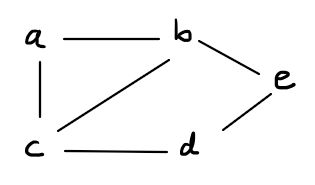
\includegraphics[height=3cm]{\pfad/Graphen/Aufgaben/adjazenzmatrix_04/adjazenzmatrix_04.png}
\begin{solutionbox}{5cm}
\begin{lstlisting}
G = [[0,1,1,0,0],
     [1,0,1,0,1],
     [1,1,0,1,0],
     [0,0,1,0,1],
     [0,1,0,1,0]]

\end{lstlisting}
\end{solutionbox}

\question[3]
In der Variablen G sei ein ungewichteter Graph als Adjazenzmatrix
implementiert.
Die Knoten a,b,c... sind auf die Indizes 0,1,2... abgebildet.
Schreibe eine Anweisung, die in der Variablen \texttt{nb} eine Liste mit
allen Buchstaben speichert, die Nachbarn von b sind.
Hinweis: die Funktion \texttt{chr(y+97)} ordnet den Zahlen y=0,1,2,... die Buchstaben
a,b,c, ... zu.

\begin{solutionbox}{2cm}
\begin{lstlisting}
nb = [chr(y+97) for y in range(len(G)) if G[1][y]]

\end{lstlisting}
\end{solutionbox}

\question[4]
Gib für den abgebildeten Graphen die Implementierung in Python als Adjazenzmatrix an.
Die Knoten a,b,c,.. sind auf die Indizes 0,1,2,... abgebildet.

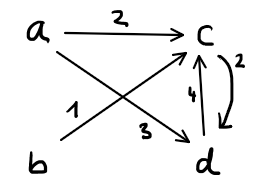
\includegraphics[height=3cm]{\pfad/Graphen/Aufgaben/adjazenzmatrix_05/adjazenzmatrix_05.png}
\begin{solutionbox}{5cm}
\begin{lstlisting}
inf = float('inf')
G = [[0,inf,2,3],
     [inf,0,1,inf],
     [inf,inf,0,2],
     [inf,inf,4,0]]

\end{lstlisting}
\end{solutionbox}

\question[3]
In der Variablen G sei ein gewichteter Graph als Adjazenzmatrix implementiert.
Die Knoten a,b,c... sind auf die Indizes 0,1,2... abgebildet.
Schreibe eine Anweisung, die in der Variablen \texttt{nb} eine Liste mit
allen Buchstaben speichert, die Nachbarn von a sind.
Hinweis: die Funktion \texttt{chr(y+97)} ordnet den Zahlen y=0,1,2,... die Buchstaben
a,b,c, ... zu.

\begin{solutionbox}{2cm}
\begin{lstlisting}
nb = [chr(y+97) for y in range(len(G)) if y != 0 and G[0][y] < inf]

\end{lstlisting}
\end{solutionbox}

\question[4]

Der gewichtete Graph G ist mit einer Adjazenzmatrix implementiert.
Die Knoten a,b,c,.. sind auf die Indizes 0,1,2,... abgebildet.
Der Floyd-Algorithmus berechnet die abgebildeten Kosten- und Wegematrizen.
Ermittle die Länge des kürzesten Weges von c nach f und gib die Länge der Teilstrecken an.
\begin{lstlisting}
(Der Punkt steht für $\infty$)
Berechnete Kostenmatrix:
0   3   .   2   4   7
.   0   .   .   1   4
1   4   0   3   5   8
.   1   .   0   2   5
.   .   .   .   0   3
.   .   .   .   .   0
Berechnete Wegematrix:
0   3   0   0   1   4
1   1   1   1   1   4
2   3   2   0   1   4
3   3   3   3   1   4
4   4   4   4   4   4
5   5   5   5   5   5
\end{lstlisting}

\begin{solutionbox}{4cm}

\begin{lstlisting}
Kürzester Weg von c nach f
(Kosten der Teilstrecken in Klammern)
c - a (1)  - d (2)  - b (1)  - e (1)  - f (3)
Gesamtkosten = 8
\end{lstlisting}
\end{solutionbox}

\question[4]
Berechne zu der Ausgangsmatrix $D^{-1}$ des Floyd-Algorithmus
die Matrix $D^3$
\begin{lstlisting}
Ausgangsmatrix: (Der Punkt steht für $\infty$)
0   .   2   7   .
1   0   4   .   12
.   .   0   1   5
.   .   .   0   3
.   .   .   .   0
\end{lstlisting}

\begin{solutionbox}{6cm}
\begin{lstlisting}
0   .   2   3   6
1   0   3   4   7
.   .   0   1   4
.   .   .   0   3
.   .   .   .   0
\end{lstlisting}
\end{solutionbox}

\question[3]
Gib für den abgebildeten Graphen die Implementierung in Python als
ein dictionary von sets an.

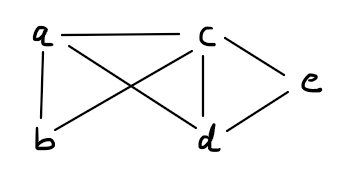
\includegraphics[height=3cm]{\pfad/Graphen/Aufgaben/ungewichtet_03/ungewichtet_03.png}
\begin{solutionbox}{5cm}
\begin{lstlisting}
G = {
'a': set('bcd'),
'b': set('ca'),
'c': set('ade'),
'd': set('ace'),
'e': set('cd')
}
\end{lstlisting}
\end{solutionbox}

\question[4]
Gib für den abgebildeten Graphen die Implementierung in Python als
ein dictionary von dictionaries an.

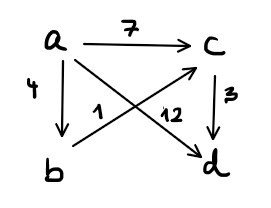
\includegraphics[height=3cm]{\pfad/Graphen/Aufgaben/gewichtet_03/gewichtet_03.png}
\begin{solutionbox}{5cm}
\begin{lstlisting}
G = {
'a': {'c':7, 'b':4, 'd':12},
'b': {'c':1},
'c': {'d':3},
'd': {}
}
\end{lstlisting}
\end{solutionbox}

\question[6]
Der gerichtete, gewichtete Graph G sei als dictionary von
dictionaries gegeben. Gehe mit Tiefensuche durch G und
speichere im Verlauf der Tiefensuche in einen dictionary \texttt{ausgangskosten} für jeden Knoten die Summe der Kosten der von ihm wegführenden Kanten.

\begin{solutionbox}{10cm}
\begin{lstlisting}
def explore(v):
    visited[v] = True
    for w in G[v]:
        ausgangskosten[v] += G[v][w]
    for w in G[v]:
        if not visited[w]:
            explore(w)

visited = {v : False for v in G}
ausgangskosten = {v: 0 for v in G}
for w in G:
    if not visited[w]:
        explore(w)

\end{lstlisting}
\end{solutionbox}

\question[3]
Der Graph wird von Startknoten a aus mit Tiefensuche traversiert. Die
  Nachbarn werden in alphabetischer Reihenfolge besucht.
  Schreibe an die Knoten ihre previsit/postvisit Nummern.

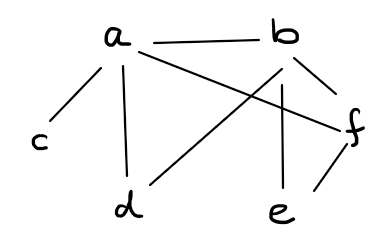
\includegraphics[height=4cm]{\pfad/Graphen/Aufgaben/visit_03/visit_03.png}

\ifprintanswers
Lösung:
\begin{lstlisting}
a  1 12
b  2  9
d  3  4
e  5  8
f  6  7
c  10 11
\end{lstlisting}
\fi

\question[4]
Der Graph wird mit dem im Unterricht vorgestellten Algorithmus topologisch
sortiert. Welche Reihenfolge ergibt sich?

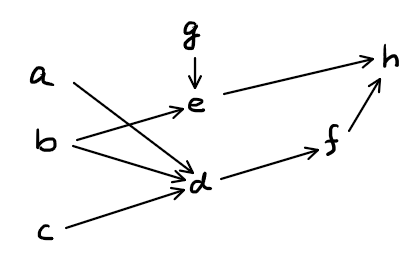
\includegraphics[height=4cm]{\pfad/Graphen/Aufgaben/toposort_03/toposort_03.png}
\begin{solutionbox}{2cm}
\begin{lstlisting}
g c b e a d f h
\end{lstlisting}
\end{solutionbox}

\question[6]
Es sollen die starken Zusammenhangskomponenten des Graphen ermittelt werden.
Der im Unterricht vorgestellte Algorithmus ermittelt dazu eine
geeignete Reihenfolge, in der die Knoten des Graphen besucht werden. Die
jeweils erreichbaren Knoten bilden dann eine starke Zusammenhangskomponente.

a. Gib diese Reihenfolge der Knoten an
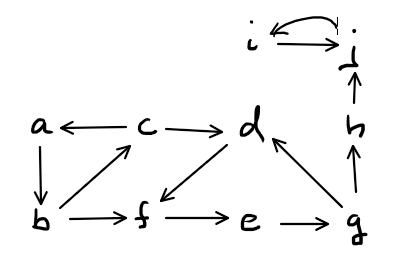
\includegraphics[height=5cm]{\pfad/Graphen/Aufgaben/scc_03/scc_03.png}
\begin{solutionbox}{2cm}
\begin{lstlisting}
i j h d g e f a c b
\end{lstlisting}
\end{solutionbox}

b. Gib die Zusammenhangskomponenten in der Reihenfolge an, wie sie von
dem im Unterricht vorgestellten Algorithmus entdeckt werden.
Die Knotenreihenfolge innerhalb einer Komponente soll
alphabetisch geordnet sein.
\begin{solutionbox}{4cm}
\begin{lstlisting}
1 - i j
2 - h
3 - d e f g
4 - a b c
\end{lstlisting}
\end{solutionbox}

\question[3]
Zeichne den shortest-path Baum der Breitensuche. Wir beginnen bei a und nehmen an,
dass Knoten auf der gleichen Ebene in alphabetischer Reihenfolge besucht werden.

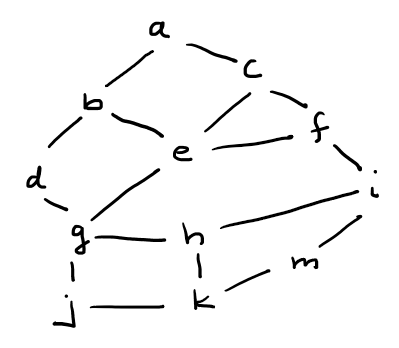
\includegraphics[height=4cm]{\pfad/Graphen/Aufgaben/breitensuche_02/breitensuche_02.png}
\begin{solutionbox}{5cm}
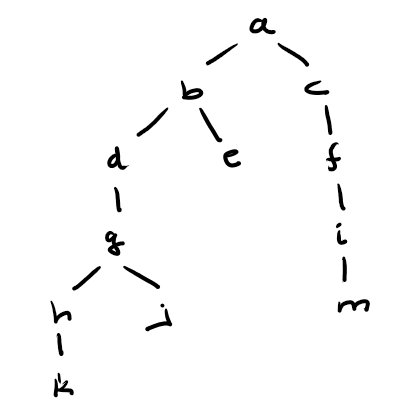
\includegraphics[height=4cm]{\pfad/Graphen/Aufgaben/breitensuche_02/breitensuche_baum_02.png}
\end{solutionbox}

\question[6]
Ermittle mit dem Algorithmus von Dijkstra die kürzesten Wege von Knoten a zu allen anderen
Knoten.  Notiere die Reihenfolge der endgültig markierten Knoten.
Notiere für jeden Knoten die Reihenfolge der Werte, mit denen er markiert wird.

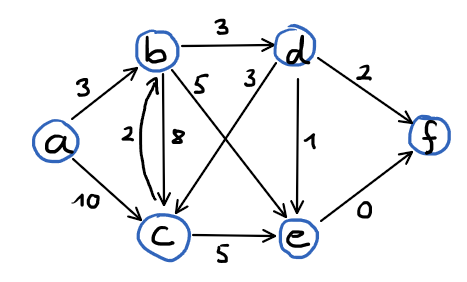
\includegraphics[height=4cm]{\pfad/Graphen/Aufgaben/dijkstra_02/dijkstra_02.png}
\begin{solutionbox}{5cm}
\begin{lstlisting}
Reihenfolge der endgültigen Markierungen: a b d e f c
a : 0
b : inf 3
c : inf 10 9
d : inf 6
e : inf 8 7
f : inf 8 7
\end{lstlisting}
\end{solutionbox}

\question[4]
Führe den Algorithmus von Bellman-Ford mit Startknoten a aus.
Notiere nach jedem Durchgang die Kosten an den Knoten

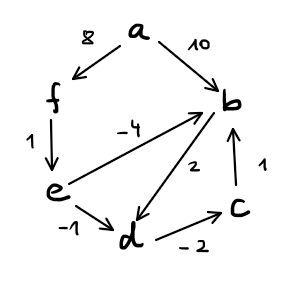
\includegraphics[height=5cm]{\pfad/Graphen/Aufgaben/bellman_03/bellman_03.png}
\begin{solutionbox}{5cm}
\begin{lstlisting}
     a  b   c   d   e   f
0 :  0  inf inf inf inf inf
1 :  0  10  10  12  9   8
2 :  0  5   10  8   9   8
3 :  0  5   5   7   9   8
4 :  0  5   5   7   9   8
\end{lstlisting}
\end{solutionbox}

\question[6]
Bestimme für den Graphen einen minimalen Spannbaum mit dem Algorithmus von Kruskal. Immer wenn der Algorithmus uns eine
Wahl lässt, wählen wir in alphabetischer Reihenfolge. Für eine Kante nennen wir die Knoten ebenfalls
in alphabetischer Reihenfolge.

a. Gib die Kanten in der Reihenfolge an, in der sie gewählt werden.  \\
b. Gib die Kosten des MST an. \\
c. Zeichne des Chefbaum des einfachen Algorithmus nach dem Verfahren aus dem Unterricht. \\
d. Zeichen den optimierten Chefbaum des Algorithmus mit path-compression und union by rank
nach dem Verfahren aus dem Unterricht.

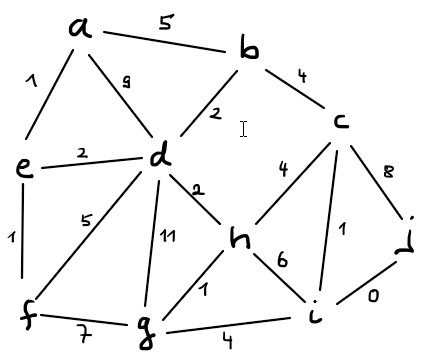
\includegraphics[height=6cm]{\pfad/Graphen/Aufgaben/kruskal_02/kruskal_02.png}
\begin{solutionbox}{9cm}
\begin{lstlisting}
i-j, a-e, c-i, e-f, g-h, b-d, d-e, d-h, b-c
Gesamtkosten:  14
\end{lstlisting}
c. 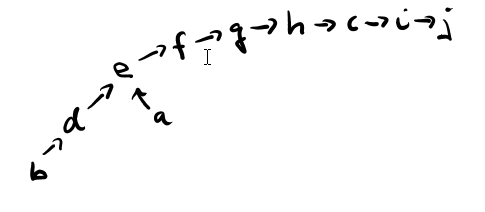
\includegraphics[height=3cm]{\pfad/Graphen/Aufgaben/kruskal_02/kruskal_02_chefbaum.png}

d. 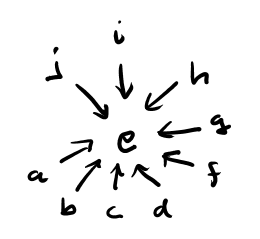
\includegraphics[height=3cm]{\pfad/Graphen/Aufgaben/kruskal_02/kruskal_02_chefbaum_opt.png}
\end{solutionbox}

\question[3]
Bestimme für den Graphen einen minimalen Spannbaum mit dem Algorithmus von Jarnik-Prim. Immer wenn der Algorithmus uns eine
Wahl lässt, wählen wir in alphabetischer Reihenfolge. Das bedeutet u.a., dass wir von Knoten a aus starten.

a. Gib die Kanten in der Reihenfolge an, in der sie gewählt werden.  \\
b. Gib die Kosten des MST an.

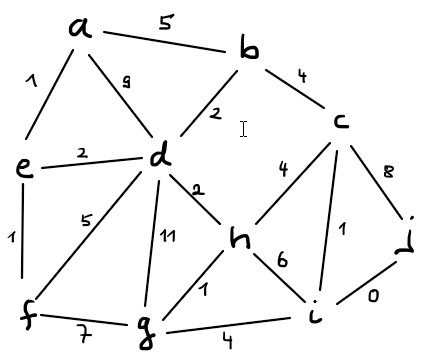
\includegraphics[height=5cm]{\pfad/Graphen/Aufgaben/prim_02/prim_02.png}
\begin{solutionbox}{3cm}
\begin{lstlisting}
a-e, e-f, e-d, d-b, d-h, h-g, b-c, c-i, i-j
Gesamtkosten:  14
\end{lstlisting}
\end{solutionbox}




% -------------------------------------------------
\end{questions}
\begin{center}
%\pointtable[h][questions]
\end{center}

\end{document}